\documentclass[a4paper,10pt]{article}
\usepackage{polski}
\usepackage[T1]{fontenc}
\usepackage[utf8]{inputenc}
\usepackage{amsfonts}
\usepackage{amsmath}
\usepackage{indentfirst}
\usepackage{graphicx}
\usepackage[scale=0.7]{geometry}
\usepackage[font=small,labelfont=bf]{caption}
\newcommand{\name}{\( \mathbb{O} \)ld-\( \mathbb{S} \)chool \( \mathbb{S} \)hooter }
\title{
	Projekt - gra \name \\
	\large Programowanie obiektowe}
\author{Michał Górniak}

\begin{document}

\maketitle

\section{Wstęp}

\name jest grą napisaną w języku Java jako projekt semestralny z programowania obiekotwego na zajęcia w Instytucie Informatyki UWr. Gra jest przeznaczona dla dwóch osób. W grze gracze toczą krótkie pojedynki w swoich statkach. Każdy pojedynek toczy się do trzech wygranych. Grafika gry jest dwuwymiarowa, a sama gra jest dość dynamiczna. Użytkownicy mają do wyboru dziewięć postaci.

\section{Instrukcja obsługi}

\subsection{Sterowanie}

\name jest sterowany wyłącznie klawiaturą. Gracz pierwszy i drugi mają osobne przyciski funkcyjne. \\

\textbf{Gracz 1:}
\begin{enumerate}
\item
sterowanie i poruszanie się po menu -- \textbf{W S A D}
\item
przycisk strzału -- \textbf{lewy ALT}
\item
przycisk ataku specjalnego -- \textbf{lewy SHIFT}
\end{enumerate}

\textbf{Gracz 2:}
\begin{enumerate}
\item
sterowanie i poruszanie się po menu -- \textbf{strzałki}
\item
przycisk strzału -- \textbf{SLASH}
\item
przycisk ataku specjalnego -- \textbf{. (PERIOD)}
\end{enumerate}

\subsection{Przebieg gry}

Po uruchomieniu programu pojawia się okienko powitalne gry. Wprost z niego gracze przechodzą do okienka wyboru tła pojedynku. Dostępne są cztery możliwe grafiki. Po wybraniu planszy gracze przechodzą do panelu wyboru postaci. Tutaj każdy gracz operuje niezależnie na swojej połówce. Użytkownik przegląda postacie i sprawdza ich statystyki. Gdy pierwszy z graczy dokona wyboru jego panel przyciemnia się i zaznacza, że ten gracz jest już gotowy do pojedynku. Rozgrywka zaczyna się, gdy drugi gracz podejmie decyzję. 

Właściwa gra polega na wygraniu jako pierwszy trzech rund. W każdej rundzie gracze zaczynają w losowym miejscu na swojej połowie planszy. Podczas rozgrywki gracze mogą dowolnie poruszać się po całej planszy i strzelać. Raz na jakiś czas gracz dostaje supermoc. Po aktywacji przyciskiem funkcyjnym wszystkie pociski wystrzelone przez gracza w przeciągu kilku sekund od aktywacji są przyspieszone i zadają podwójne obrażenia. Gracze podczas pojedynku mogą także łapać losowo spadające serca, aby zregenerować swoje zdrowie. Nie mogą jednak uzyskać więcej zdrowia, niż mieli na początku rundy. Punkt za rundę zdobywa gracz, który zabierze jako pierwszy całe życie drugiego gracza. W przypadku remisu obaj gracze zdobywają punkt.

\section{Analiza obiektowa}
\subsection{Lista klas z opisem}
\subsubsection{Frame}

Klasa dziedzicząca po \textit{JFrame}. Ustawia domyślne wartości dla okna (resizable(false), wymiary, wyjście).

\subsubsection{BackgroundFrame}

Okno wyboru tła. Dziedziczy po \textit{Frame}. Ma w sobie tylko jeden panel \textit{BackgroundPanel}.

\subsubsection{BackgroundPanel}

Panel wybrou tła. Na ekranie pojawiają się cztery prostokąty z pomniejszonymi grafikami do wyboru. Wybieramy tło poruszając się klawiszami ruchu i zatwierdzamy przyciskiem funkcyjnym. Aktywne w danym momencie tło jest podświetlone, a jego przyciemniona wersja jest widoczna w tle.

\begin{center}
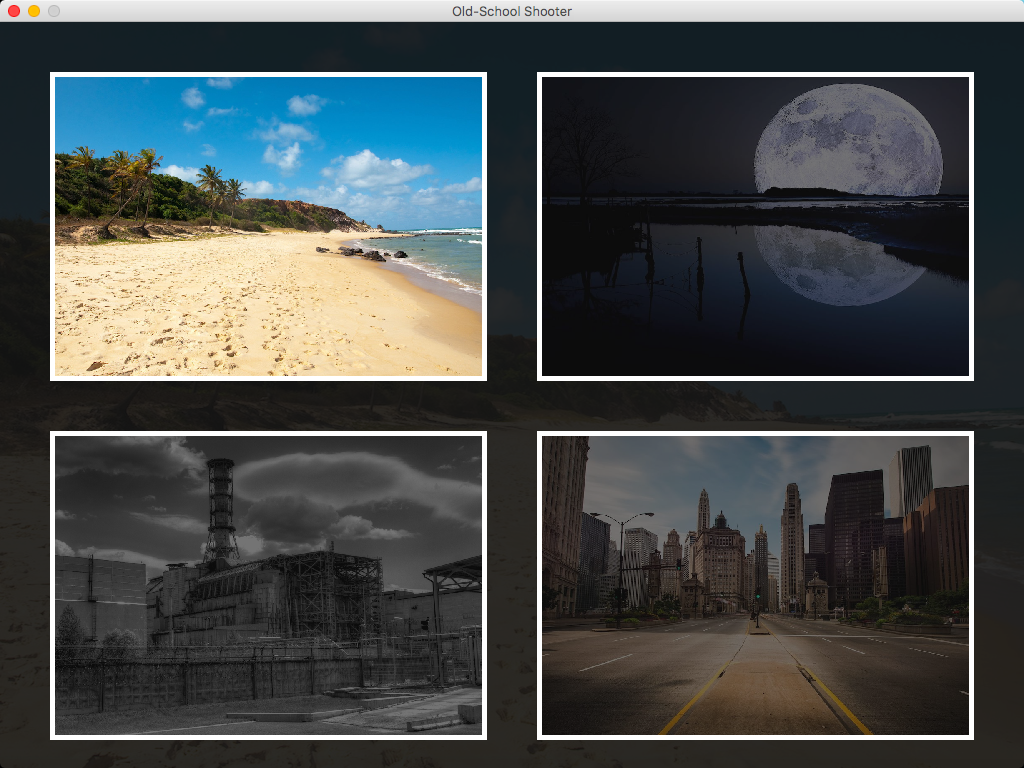
\includegraphics[scale=0.18]{tlo.png}
\captionof{figure}{Panel wyboru tła.}
\end{center}

\subsubsection{BoardFrame}

Okno rozgrywki (planszy). Dziedziczy po \textit{Frame}. Ma w sobie tylko jeden panel \textit{BoardPanel}.

\subsubsection{BoardPanel}

Panel rozgrywki. Zaimplementowanie przy użyciu głownie rysowania planszy, wstawiania obrazków i ustawiania różnych timerów. W rozgrywce występują też czynniki losowe. Spadające serca pojawiają się w losowym miejscu, gracze startują na losowych pozycjach na swoich połowach. Co określoną stałą plansza odświeża się, przerysowując wszystko od nowa, co tworzy efekt animacji. W klasie tej trzymani są bohaterowie. W górnej części panelu mieszczą się stany zdrowia bohaterów oraz aktualny wynik. Przed każdą rundą pojawia się animacja odliczania do rozpoczęcia rundy. Po zakończeniu ostatniego pojedynku pojawia się animacja \textit{Game Over}.

\begin{center}
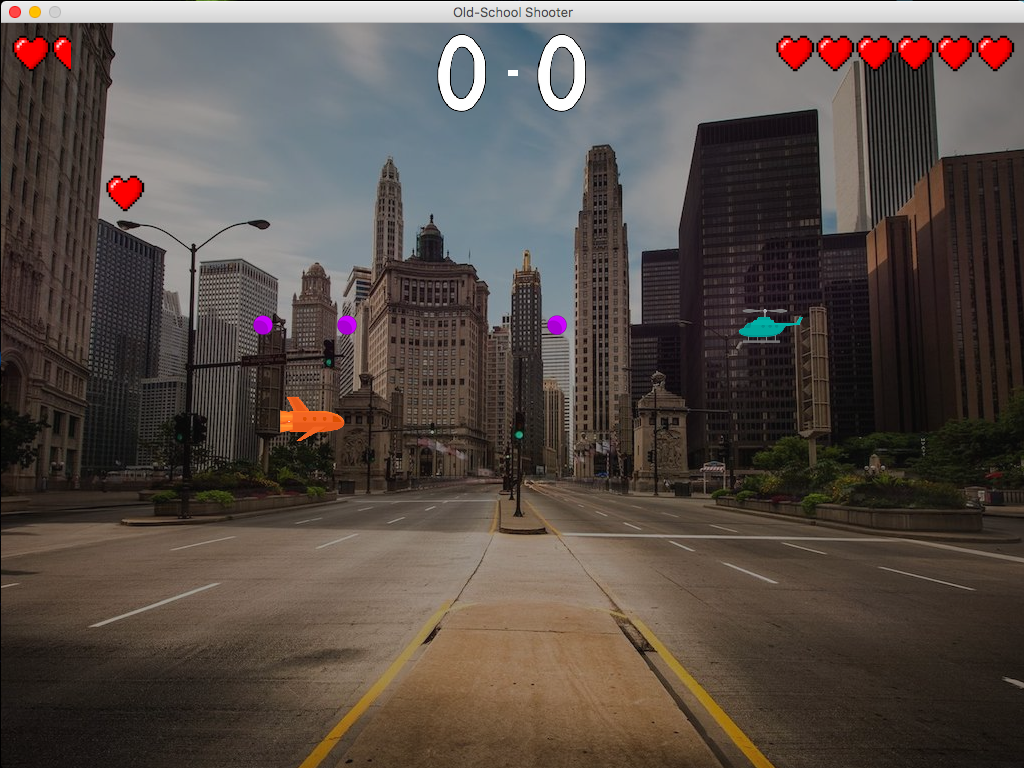
\includegraphics[scale=0.18]{pojedynek.png}
\captionof{figure}{Panel pojedynku.}
\end{center}

\subsubsection{CharacterFrame}

Okno wyboru postaci. Dziedziczy po \textit{Frame}. Ma w sobie tylko jeden panel \textit{CharacterPanel}.

\subsubsection{CharacterPanel}

Panel wyboru postaci. Są to dwie kopie (na odpowiednich połowach) menu wyboru postaci (dla gracza lewego i prawego). W górnej części pojawia się aktualnie zaznaczona postać i jej statystyki. W dolnej części jest panel wyboru bohatera. Gracze w tej części wybierają niezależnie. Gdy jeden z graczy dokona wyboru jego okienko przyciemnia się i wyświetlany jest komunikat \textit{Ready}. Menu zostało to zaimplementowane jako grafiki i rysowanie prostych obiektów, a przyski są tak naprawdę przemalowywane za każdym razem, gdy któryś z graczy wciśnie odpowiedni klawisz. Dla uatwienia implementacji w klasie jest funkcja rysująca połowę ekranu (z odpowiednimi parametrami).

\begin{center}
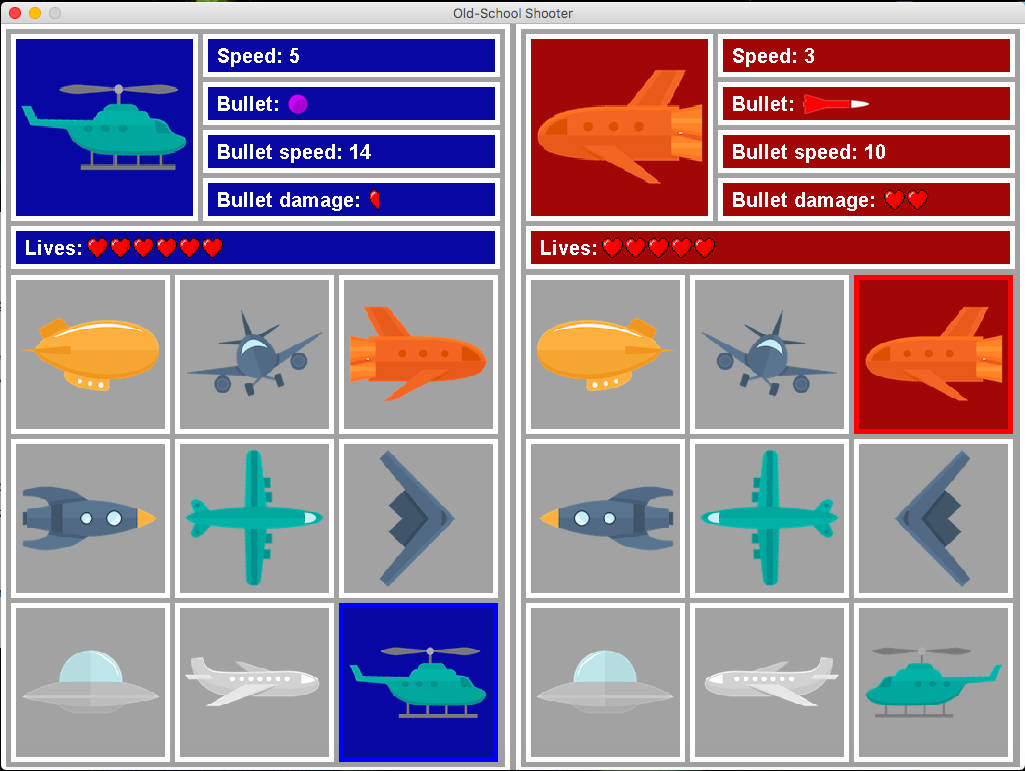
\includegraphics[scale=0.18]{postacie.png}
\captionof{figure}{Panel wyboru postaci.}
\end{center}

\subsubsection{GameOverFrame}

Okno uruchamiane po zakończeniu pojedynku. Dziedziczy po \textit{Frame}. Ma w sobie tylko jeden panel \textit{GameOverPanel}.

\subsubsection{GameOverPanel}

Prosty panel uruchamiany po zakończeniu gry. Jest na nim popularna grafika \textit{Game Over} oraz wynik pojedynku i miniaturki graczy. Dostępne są dwa przyciski: jeden do powrotu do menu głównego, a drugi do zakończenia gry.

\begin{center}
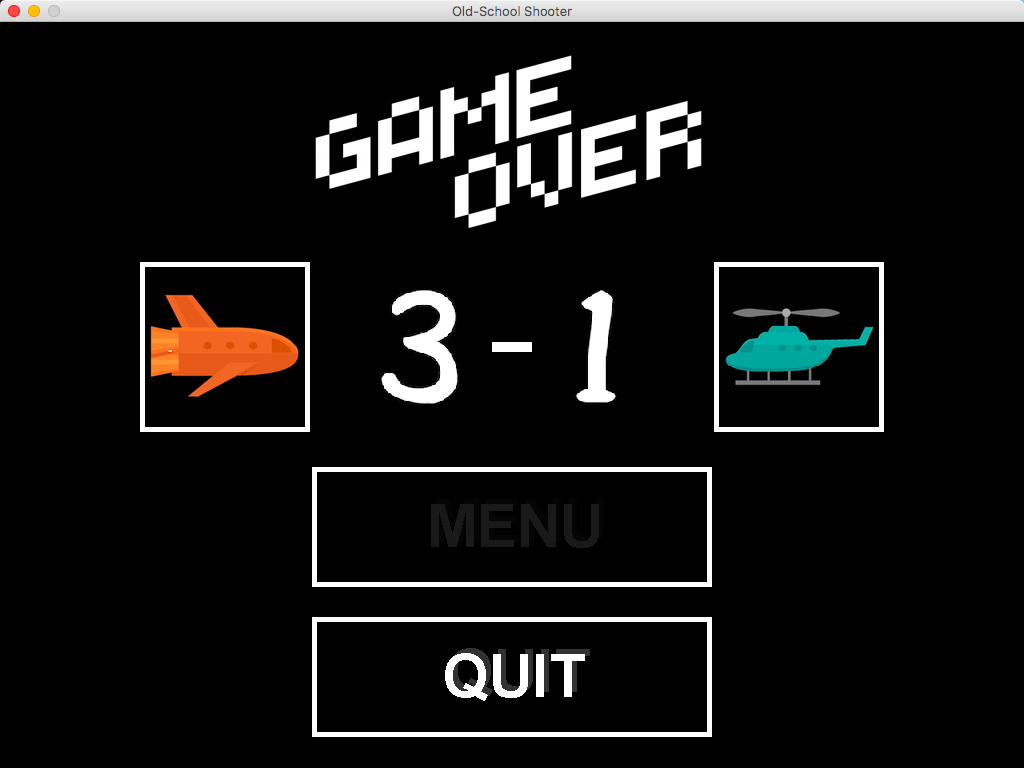
\includegraphics[scale=0.18]{gameover.png}
\captionof{figure}{Panel \textit{Game Over}.}
\end{center}

\subsubsection{MenuFrame}

Okno uruchamiane przy starcie programu. Dziedziczy po \textit{Frame}. Ma w sobie tylko jeden panel \textit{MenuPanel}.

\subsubsection{MenuPanel}

Panel startowy. Za każdym uruchomieniem pojawia się losowe tło. Co kilka sekund zmieniają się miniaturki po lewej i prawej stronie oraz ich pozycje. Zmienia się także kolor napisu na przycisku \textit{New game}.

\begin{center}
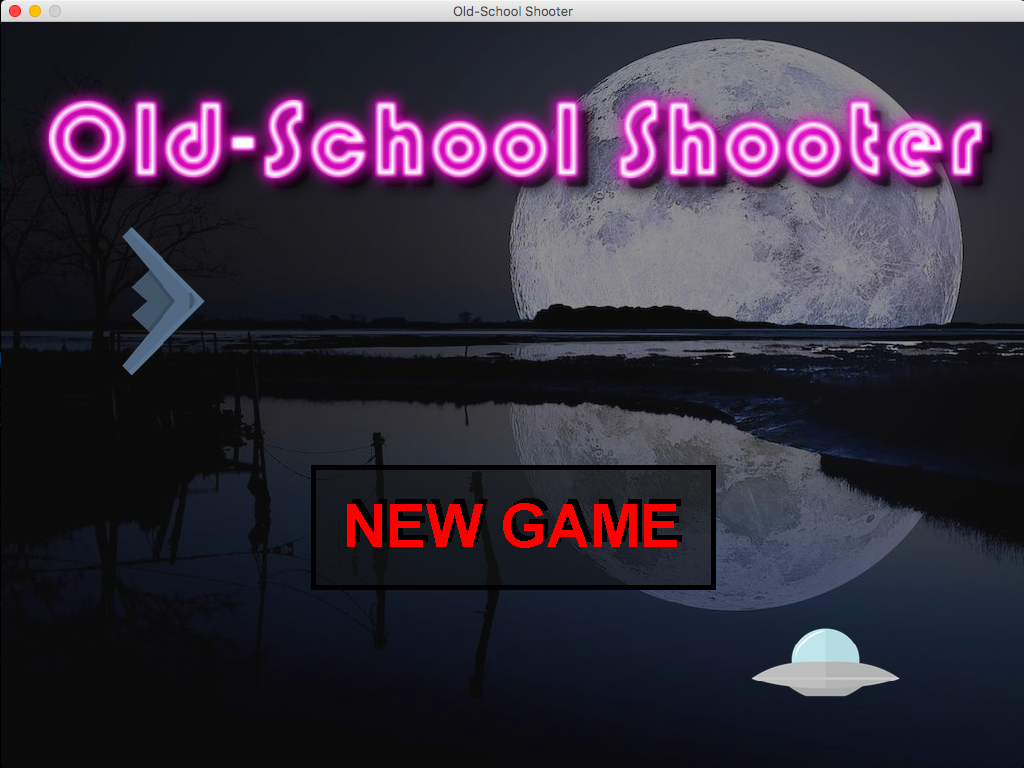
\includegraphics[scale=0.18]{menu.png}
\captionof{figure}{Panel menu.}
\end{center}

\subsubsection{MovingCharacter}

Klasa zawierająca podstawowe wartości dla poruszającego się po planszy obiektu (np. koordynaty, obrazek).

\subsubsection{Hero}

Klasa bohatera. Dziedziczy po \textit{MovingCharacter}. Zawiera metody poruszania się bohatera oraz trzyma jego aktualne zdrowie, szybkość, a także listę wystrzelonych przez niego pocisków.

\subsubsection{Bullet}

Klasa pocisku. Dziedziczy po \textit{MovingCharacter}. Zawiera prędkość posicku.

\subsubsection{Superbullet}

Podklasa pocisku. Pociski te zadają podwójne obrażania oraz są dodatkowo przyspieszone.

\subsubsection{FallingLife}

Klasa implementująca losowo spadające serca podczas rozgrywki.

\subsubsection{GameConst}

Klasa z ustawieniami gry. Jest to klasa z prywatnym konstruktorem i publicznymi finalnymi statycznymi zmiennymi.

\subsubsection{HeroStats}

Klasa ze statystykami bohaterów oraz ich pocisków.

\subsubsection{MyImage}

Pomocnicza klasa do obsługi obrazów. Trzyma obiekt klasy Image oraz pola i metody potrzebne do wygodnej obsługi obrazu.

\subsubsection{Main}

Klasa uruchamiająca program.
\newpage
\subsection{Diagram klas}
Poniżej przedstawiam diagram klas projektu: \\ \\
\begin{center}
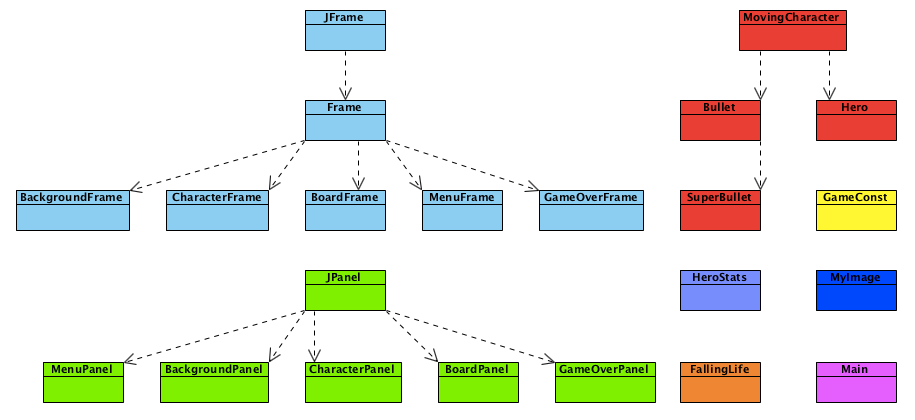
\includegraphics[width=\textwidth]{klasy.png}
\captionof{figure}{Diagram klas.}
\end{center}
\subsection{Realizowana funkcjonalność}
\subsubsection{Użytkownik}
Każdy użytkownik ma taki sam dostęp do aplikacji. W grze nie zostały umieszczone żadne ukryte umiejętności, które faworyzują któregoś z graczy. Rozgrywka jest symetryczna dla obu graczy. Każdy użytkownik ma zatem dostęp do wszystkich funkcji programu.
\subsubsection{Programista}
Aplikacja jest przystosowana do dalszego rozwoju. Więcej o tym w rozdziale \textbf{Dalsza rozbudowa}. Poza rozszerzeniem kodu użytkownik może dowolnie zmieniać grafiki postaci i tła podmieniając odpowiednie pliki w folderze \textit{images}. Poza tym programista może modyfikować klasy \textit{GameConst} i \textit{HeroStats}, aby dopasować statystki postaci i ustawienia gry do własnych upodobań i testów.
\section{Dalsza rozbudowa}
Gra była pisana w dość krótkim czasie, istnieje zatem wiele możliwości rozwoju. Programista ma w tym przypadku pozostawioną dużą dowolność. Modyfikacje można rozpocząć od zmiany statystyk i ustawień gry. Nietrudno też dodać nowe strzały i ataki specjalne. Dla przykładu strzały można rozbudowywać tworząc podklasy klasy \textit{Bullet}, dodając im nowe grafiki i zmieniając parametry lub sposób działania. Grę można też rozszerzyć o dodatkowe postacie, a postaciom tym można dodać nowe umiejętności.
\end{document}